\documentclass{lab1report}
\usepackage{float}
% 封面信息：只需修改下面各项。
\course{网络安全}
\reporttitle{实验报告}
\student{江李阳(学号:202400460042)，王健一(学号:202400460039)，邱泽辉(学号:202400460046)}
\instructor{郭山清}
\college{网络空间安全学院}
\major{密码科学与技术2024级一班}
\completiondate{2026 年  9月  10日}

% 参考资料写入 references.bib；直接引用使用 \labquote[页码]{文献键}。
\addbibresource{references.bib}

\begin{document}
\makecover

% 公共章节：按实验报告要求保留，正文由作者自行填写。
\section{实验目标}
\begin{itemize}
    \item 通过实验操作和网络流量分析，深入理解交换机和路由器的工作原理。
    \item 掌握子网划分和子网掩码的概念和应用，理解子网掩码在网络通信中的重要性。
    \item 熟练使用tcpdump工具，掌握获取和分析网络流量的技能。
    \item  为后续章节的学习和深入理解网络原理奠定基础，提升解决实际网络问题的能力。
\end{itemize}
% 在此填写实验目标。
% 在此填写实验原理。
\section{实验原理}
\subsection{ARP}
ARP(Address Resolution Protocol,地址解析协议)，用于将IP地址解析为MAC地址。因为以太网通信时除了知道IP地址外，还需要知道下一跳的MAC地址，才能发送以太网帧。比如
A与B通信时，A希望给B发送以太网帧，就必须知道B的MAC地址，如果A,B不在同一个网段，那么A需要知道网关的MAC地址。

当发送IP数据包时，主机先查询自己的ARP缓存表，如果已经有目标IP和MAC的映射，则直接使用该映射发送以太网帧(IP数据包封装在以太网帧中)。如果没有，则需要先构造ARP请求，具体过程如下:
\begin{itemize}
    \item ARP请求时发送广播帧，源MAC地址为A的MAC地址，目的MAC地址为$\texttt{FF:FF:FF:FF:FF:FF}$即广播帧；以太网类型为$\texttt{0x0806}$表示ARP；操作码为1，表示请求；源IP地址为A的IP地址；ARP报文中的目标硬件地址字段为全0(因为此时还不知道目标MAC地址)，目的IP地址为要解析的IP地址，如B的IP或网关IP。
    \item 交换机收到广播帧后会向同一广播域内的其他端口泛洪，因此同一局域网内的主机都会收到该ARP请求的广播帧，但只有目标IP匹配的主机才会处理该请求，其他主机直接丢弃。
    \item 目标主机(或网关)发现所问的就是自己时，首先会更新自身的ARP缓存，记录请求方的IP和MAC地址；接着构造ARP响应，操作码为2，该回复的以太网帧的目的MAC是请求方MAC，即以单播回复。
    \item A收到ARP响应后将对应的下一跳IP与下一跳的MAC对应关系记录下来，写入ARP缓存中。
\end{itemize}

\subsection{ICMP}
ICMP(Internet Control Message Protocol,互联网控制报文协议)属于网络层协议，但封装在IP包中，IPv4首部中的协议号为1表示上层协议为ICMP。它不是面向应用的数据传输协议，主要用于报告错误、网络诊断和路由控制等。
常见类型包括：
\begin{itemize}
    \item 查询类报文：Echo Request的Type为8，用于请求目标主机回应；Echo Reply的Type为0，用于回应Echo Request。
\end{itemize}

差错类报文及其常见用途如下，其中Redirect报文会在子网掩码配置错误的实验中出现：
\begin{table}[htbp]
    \centering
    \caption{常见ICMP差错类报文}
    \label{tab:icmp-error-types}
    \begin{tabular}{ccc}
        \toprule
        类型 & 名称 & 用途 \\
        \midrule
        3  & Destination Unreachable & 目标不可达 \\
        4  & Source Quench & 源抑制，已废弃 \\
        5  & Redirect & 重定向，告知主机有更好的下一跳 \\
        11 & Time Exceeded & 超时，TTL减到0或分片重组超时 \\
        12 & Parameter Problem & IP头部字段问题 \\
        \bottomrule
    \end{tabular}
\end{table}

Type 3和Type 11报文中常见的Code字段含义如下：
\begin{table}[htbp]
    \centering
    \caption{ICMP Type 3的常见Code}
    \label{tab:icmp-type3-code}
    \begin{tabular}{cc}
        \toprule
        Code & 含义 \\
        \midrule
        0 & 网络不可达 \\
        1 & 主机不可达 \\
        2 & 协议不可达 \\
        3 & 端口不可达 \\
        4 & 需要分片但DF位置位 \\
        5 & 源路由失败 \\
        \bottomrule
    \end{tabular}
\end{table}

\begin{table}[htbp]
    \centering
    \caption{ICMP Type 11的常见Code}
    \label{tab:icmp-type11-code}
    \begin{tabular}{cc}
        \toprule
        Code & 含义 \\
        \midrule
        0 & TTL超时 \\
        1 & 分片重组超时 \\
        \bottomrule
    \end{tabular}
\end{table}

\subsection{Ping}
Ping的本质是发送$\texttt{ICMP Echo Request}$，等待对方回复$\texttt{ICMP Echo Reply}$，计算往返时间RTT。Ping并不使用TCP/UDP，因此没有端口，而是直接使用ICMP。
Ping的完整流程如下(假设A Ping B):
\begin{itemize}
    \item 解析目标IP：A执行$\texttt{ping test.com}$，此时Ping的目标如果是域名，系统先会做DNS解析，得到对应的IP；如果Ping的是IP，则直接使用。
    \item 构造ICMP报文(Type=8，类型为Echo Request)：封装进IP包，加上IP头部信息，包括源IP(A的IP地址)和目的IP(B的IP地址)，协议号为1表示ICMP。
    \item 封装IP包：发送前必须知道下一跳MAC，如果是B在相同子网下，下一跳就是B，ARP解析出B的MAC地址（查ARP缓存或构造ARP请求）；如果B与A不在同一子网，即跨网段了，则ARP解析网关的MAC地址。最终封装成以太网帧并发出。
    \item 网络转发：若B与A在相同子网，则由交换机根据MAC和端口映射关系直接转发；若不在同一子网，则由路由器转发，经过路由器时会去掉原来的以太网帧头，将其中的IP包部分字段做修改(如TTL值减一、重新计算校验和等)，查询路由表确认下一跳IP地址以及对应MAC地址，重新封装以太网帧(如果TTL减为0，路由器直接丢包，并返回ICMP Time Exceeded)。
    \item 收到ICMP请求：当B收到IP包后，检查发现目的IP的确是自身且协议是ICMP(类型8，Echo Request)，然后B将构造Echo Reply并将该回复发送给A(该过程同样要经历查ARP并发送给下一跳)。
    \item 收到ICMP回复：当A收到Echo Reply后会先检查ICMP校验和、检查序号等参数与之前的请求相匹配，然后用收到时间减去发送时的时间计算RTT。
\end{itemize}



\section{实验设置}
% 在此填写 VMware、OpenWRT、网卡、地址和工具版本等实验设置。

% 三个任务分别维护在 content/ 目录中。
\input{content/task1}
% 实验二：使用 Wireshark 分析 Web 访问过程流量
% 在此填写 DNS、ARP、TCP、HTTP、Follow TCP Stream 和 Cookie 分析。
\section{实验二：使用 Wireshark 分析 Web 访问过程流量}

\subsection{实验目的}
\begin{enumerate}
    \item 学习并掌握Wireshark在网络流量分析中的作用，以及如何通过它来捕获和分析网络数据包;
    \item 通过实际操作，观察并分析域名解析过程中涉及的IP包，理解DNS请求和响应的格式和内容,以及它是如何将域名转换为IP地址的;
    \item 观察并解释Client与www.imool.com.cn之间TCP连接的建立和拆除过程，包括三次握手和四次挥手;
    \item 使用Wireshark的协议流追踪功能，提取并分析Web访问过程中产生的Cookie信息
\end{enumerate}

\subsection{实验配置}
本次实验采用 Oracle VirtualBox 搭建实验环境，OpenWRT路由器通过三个接口分别和Client、Web Server、DNS相连，具体网络拓扑的配置如下：
\begin{table}[H]
    \centering
    \caption{实验二各虚拟机网络接口及 IP 地址配置}
    \label{tab:exp2_network}
    \begin{tabular}{cccc}
        \toprule
        虚拟机 & Linux 内网卡名 & IP 地址 & 默认网关 \\
        \midrule
        Client      & \texttt{enp0s3} & \texttt{192.168.3.10/24}  & \texttt{192.168.3.1} \\
        DNS Server  & \texttt{enp0s3} & \texttt{192.168.2.53/24}  & \texttt{192.168.2.1} \\
        Web Server  & \texttt{enp0s3} & \texttt{192.168.4.105/24} & \texttt{192.168.4.1} \\
        OpenWRT     & \texttt{eth1}   & \texttt{192.168.4.1/24}   & -- \\
        OpenWRT     & \texttt{eth2}   & \texttt{192.168.3.1/24}   & -- \\
        OpenWRT     & \texttt{eth3}   & \texttt{192.168.2.1/24}   & -- \\
        OpenWRT     & \texttt{eth0}   & DHCP                      & -- \\
        \bottomrule
    \end{tabular}
\end{table}
网络拓扑如图所示：
\begin{figure}[H]
    \centering
    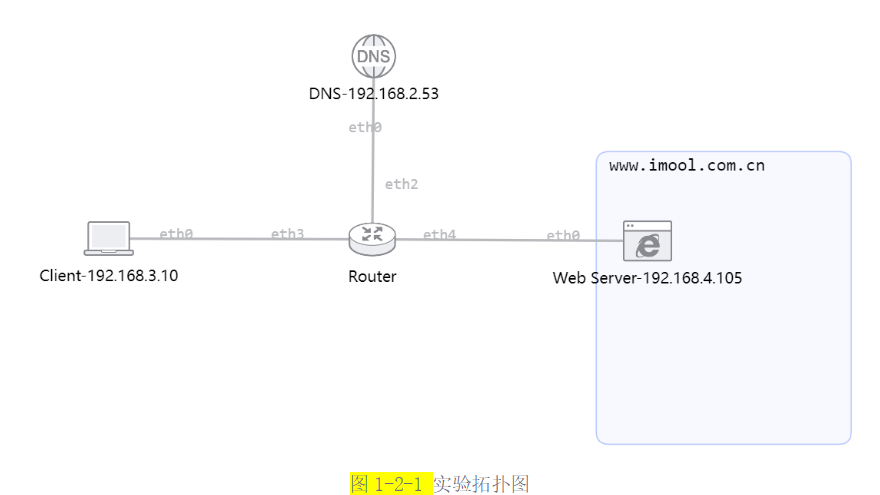
\includegraphics[width=0.8\textwidth]{figures/exp2_network.png}
    \caption{实验二网络拓扑图}
    \label{fig:exp2_network}
\end{figure}
\subsection{实验过程}
\subsubsection{配置 Web Server}
在 Web Server 主机 192.168.4.105 上启动 HTTP 服务。
由于系统中未安装 Apache 或 Nginx，因此使用 Python 自带的 HTTP Server 建立简单的 Web 服务。
执行：
\begin{lstlisting}[language=bash,caption={建立简单的 Web 服务}]
sudo python3 -m http.server 80 --bind 0.0.0.0
ss -lntp
\end{lstlisting}
查看端口监听状态，可以看到 0.0.0.0:80 已处于监听状态，
说明 Web Server 已成功提供 HTTP 服务。
\begin{figure}[H]
    \centering
    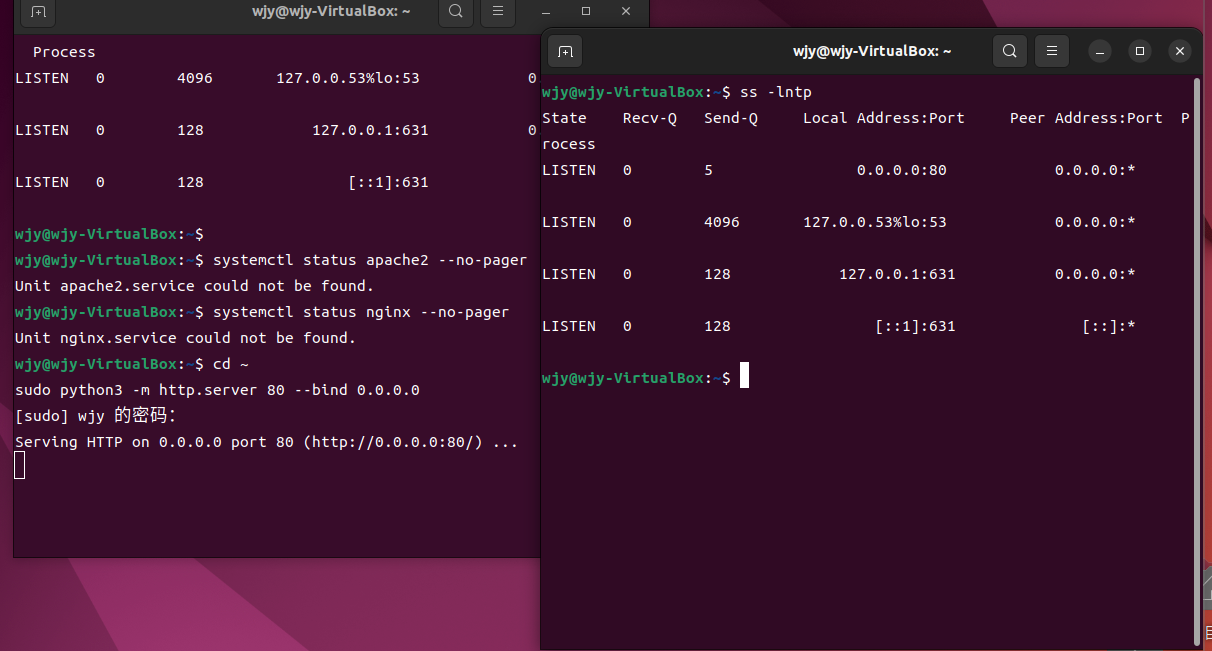
\includegraphics[width=0.8\textwidth]{figures/exp2_http.png}
    \caption{Web Server 启动 HTTP 服务截图}
    \label{fig:exp2_http}
\end{figure}

\subsubsection{配置 DNS Server}
在虚拟机DNS Server上打开终端，使用nano编辑器创建配置文件：
\begin{lstlisting}[language=bash,caption={创建DNS配置文件}]
cat > ~/imool-dnsmasq.conf <<'EOF'
listen-address=192.168.2.53
bind-interfaces
address=/www.imool.com.cn/192.168.4.105
no-resolv
EOF  
\end{lstlisting}
检查配置文件的语法，如下：
\begin{lstlisting}[language=bash,caption={检查DNS配置文件语法}] 
sudo dnsmasq --test --conf-file="$HOME/imool-dnsmasq.conf"
\end{lstlisting}
在确认后，启用DNS服务，如下：
\begin{lstlisting}[language=bash,caption={启用DNS服务}]
sudo dnsmasq --no-daemon --conf-file="$HOME/imool-dnsmasq.conf"
\end{lstlisting}

此时 DNS Server 可以响应 Client 对 www.imool.com.cn 的解析请求，
并返回 Web Server 的 IP 地址 192.168.4.105。
\begin{figure}[H]
    \centering
    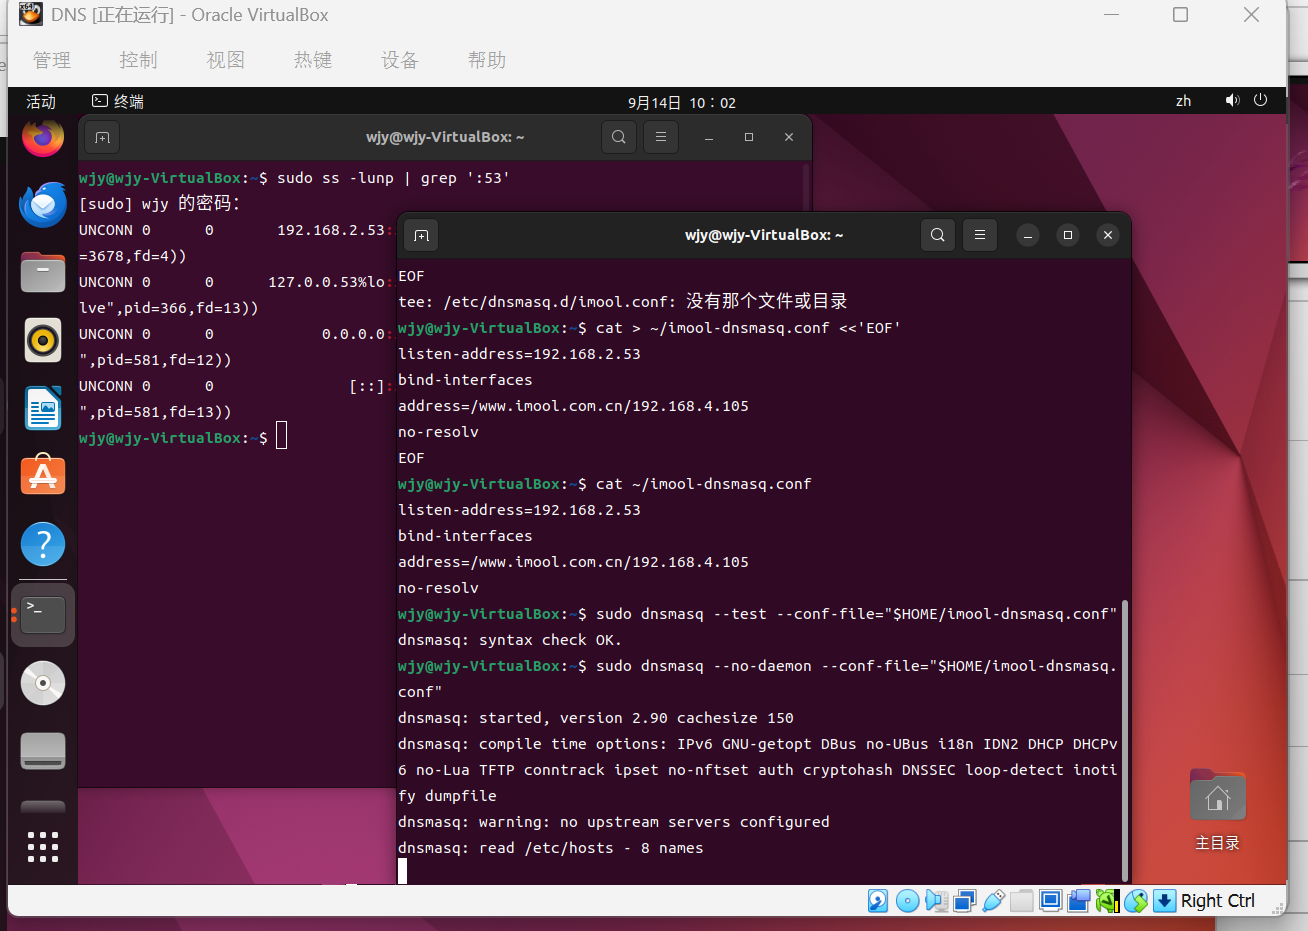
\includegraphics[width=0.8\textwidth]{figures/exp2_dns.png}
    \caption{DNS Server 启动截图}
    \label{fig:exp2_dns}
\end{figure}

\subsubsection{配置 Client 并启动 Wireshark}
在 Client 上启动 Wireshark，并选择 enp0s3 接口监听网络流量。
为尽可能完整地观察 ARP 和 DNS 解析过程，在访问网站前清除相关缓存：
\begin{lstlisting}[language=bash,caption={清除 DNS 缓存}]
sudo ip neigh flush all
sudo resolvectl flush-caches
\end{lstlisting}
之后开始 Wireshark 抓包:
\begin{lstlisting}[language=bash,caption={启动 Wireshark 抓包}]sudo wireshark &
sudo wireshark
\end{lstlisting}

在Client上先运行Wireshark，选择监听以太网网卡eth0的所有流量；
在Client上通过浏览器访问$$ http://www.imool.com.cn $$，然后结束访问该网站；
\begin{figure}[H]
    \centering
    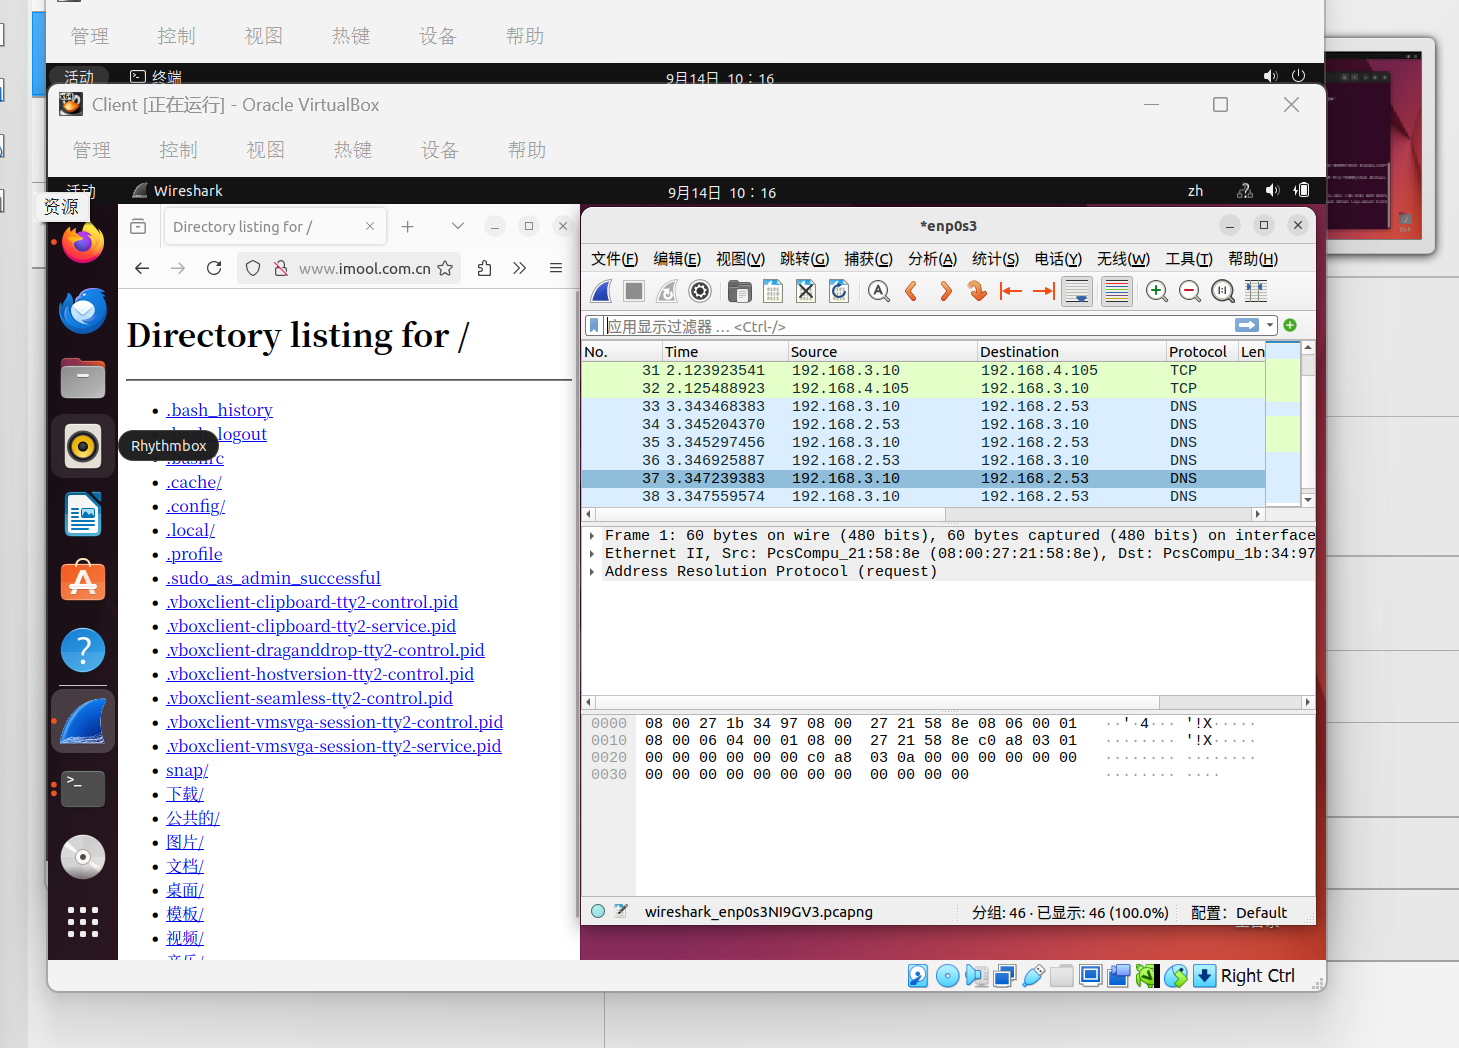
\includegraphics[width=0.8\textwidth]{figures/exp2_wireshark.png}
    \caption{Wireshark抓包截图}
    \label{fig:exp2_wireshark}
\end{figure}


\subsubsection{抓取相关的协议流量}
抓取相关的DNS流量，如下：
\begin{figure}[H]
    \centering
    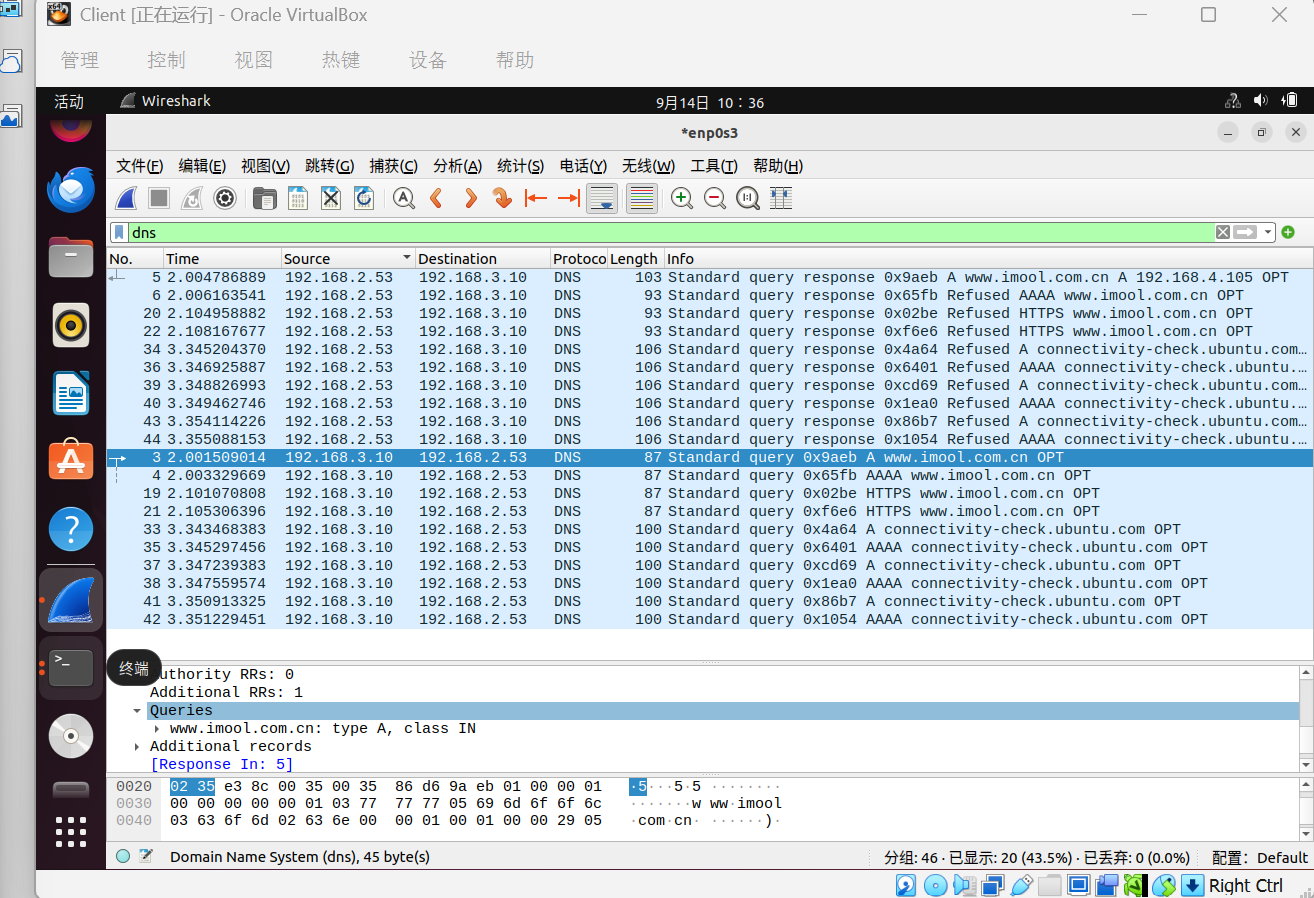
\includegraphics[width=0.8\textwidth]{figures/exp2_dns_1.png}
    \caption{DNS流量截图1}
    \label{fig:exp2_dns_1}
\end{figure}

\begin{figure}[H]
    \centering
    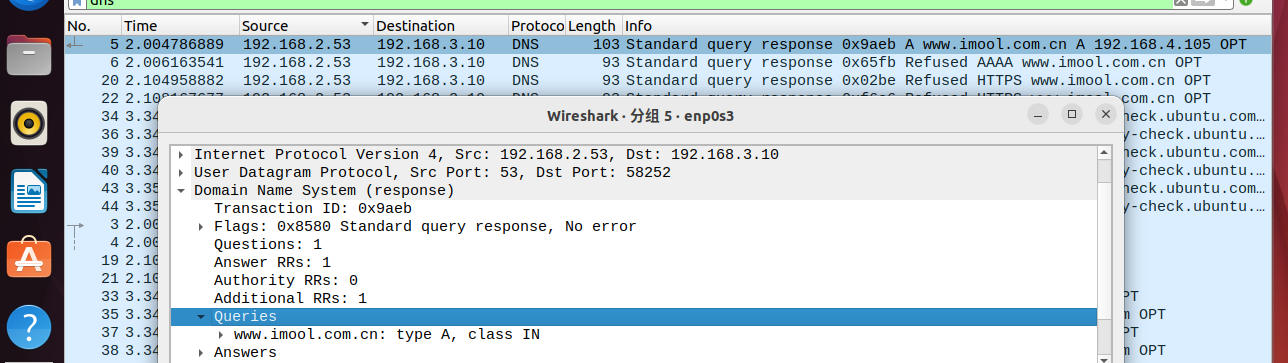
\includegraphics[width=0.8\textwidth]{figures/exp2_dns_2.png}
    \caption{DNS流量截图2}
    \label{fig:exp2_dns_2}
\end{figure}

抓取相关的ARP流量，如下：
\begin{figure}[H]
    \centering
    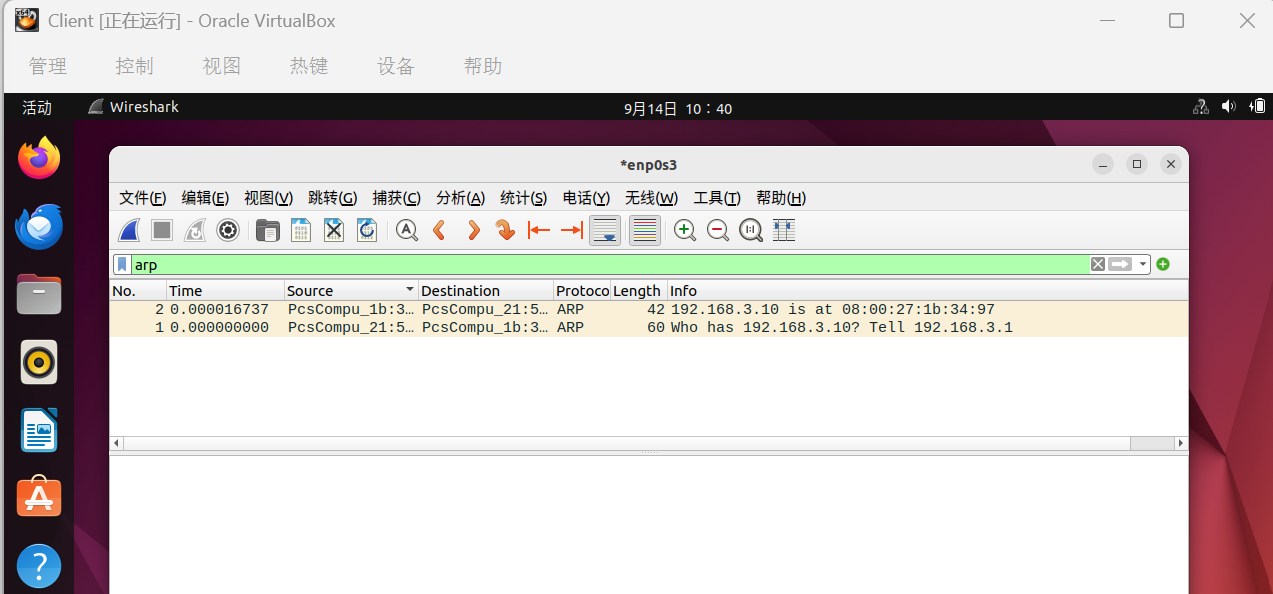
\includegraphics[width=0.8\textwidth]{figures/exp2_arp.png}
    \caption{ARP流量截图}
    \label{fig:exp2_arp}
\end{figure}

抓取相关的TCP流量，如下：
\begin{figure}[H]
    \centering
    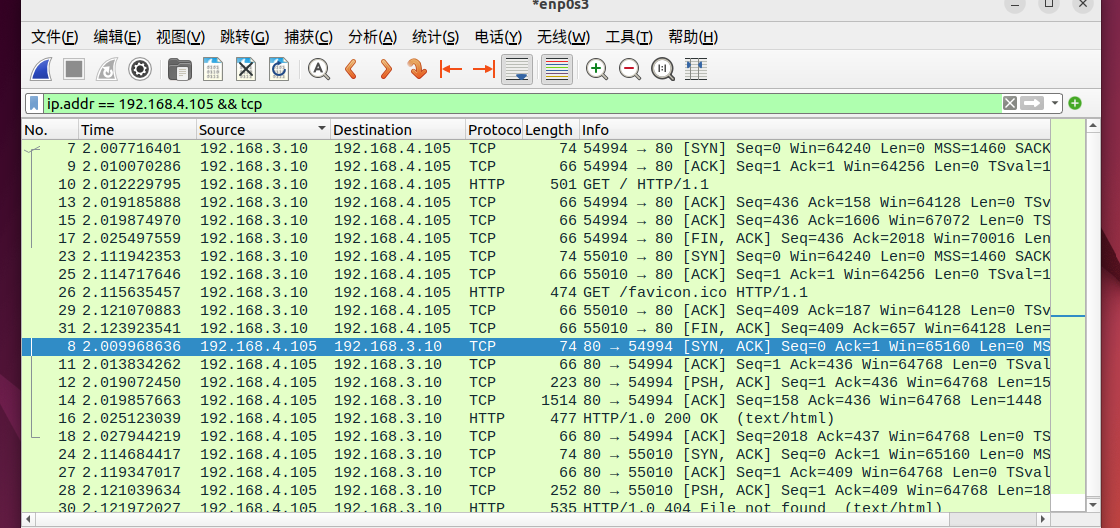
\includegraphics[width=0.8\textwidth]{figures/exp2_tcp.png}
    \caption{TCP流量截图}
    \label{fig:exp2_tcp}
\end{figure}

抓取相关的HTTP流量，如下：
\begin{figure}[H]
    \centering
    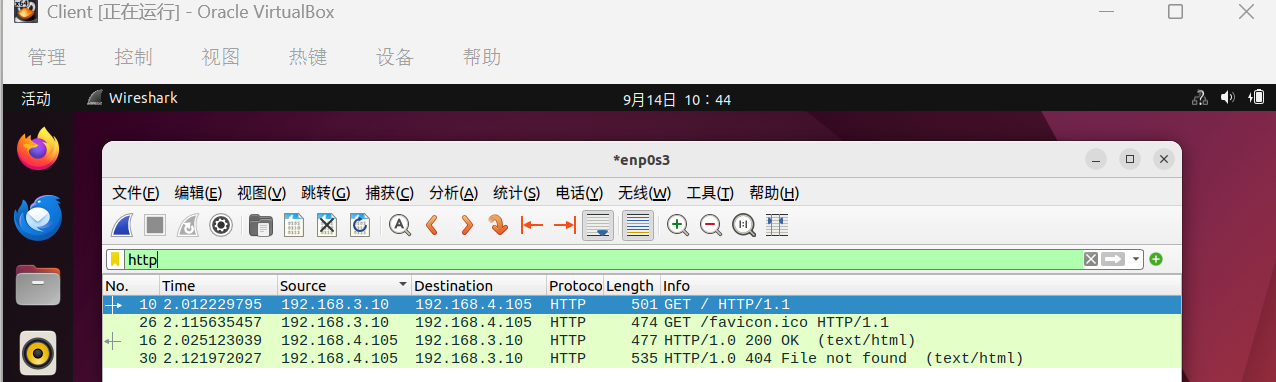
\includegraphics[width=0.8\textwidth]{figures/exp2_http_1.png}
    \caption{HTTP流量截图1}
    \label{fig:exp2_http_1}
\end{figure}

\begin{figure}[H]
    \centering
    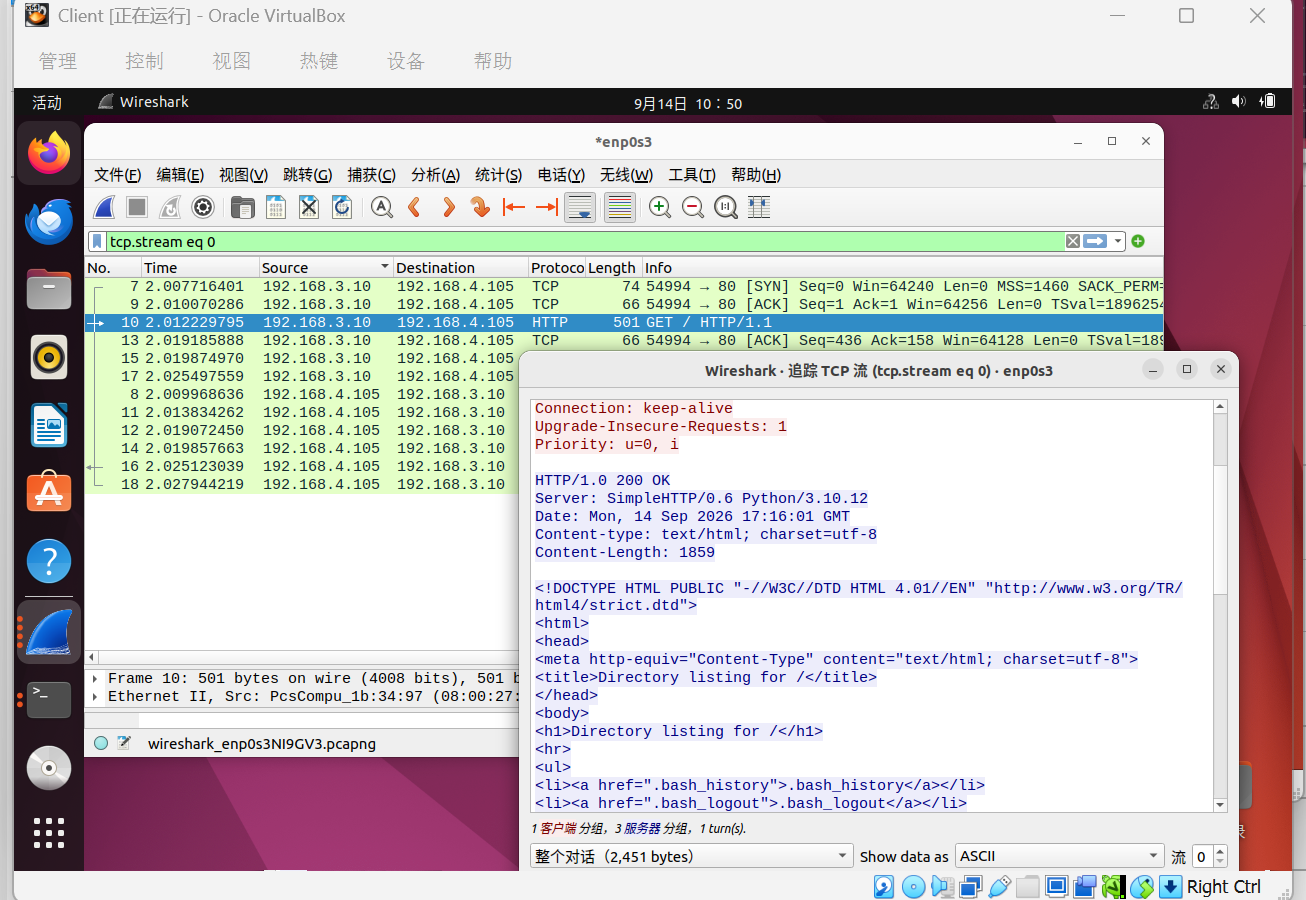
\includegraphics[width=0.8\textwidth]{figures/exp2_http_2.png}
    \caption{HTTP流量截图2}
    \label{fig:exp2_http_2}
\end{figure}

发现上述图片中没有cookie，于是自己手写添加一个，
创建一个简单的服务器：
\begin{lstlisting}[language=python,caption={创建简单的服务器}]
nano ~/cookie_server.py
\end{lstlisting}
写入：
\begin{lstlisting}[language=python,caption={写入简单的服务器}]
from http.server import HTTPServer, SimpleHTTPRequestHandler

class CookieHandler(SimpleHTTPRequestHandler):
    def end_headers(self):
        self.send_header("Set-Cookie", "username=wjy; Path=/")
        super().end_headers()

server = HTTPServer(("0.0.0.0", 80), CookieHandler)

print("HTTP server running on port 80...")
server.serve_forever()
\end{lstlisting}
保存以后运行：
\begin{lstlisting}[language=bash,caption={运行简单的服务器}]
sudo python3 ~/cookie_server.py
\end{lstlisting}

最后重新执行：
wireshark抓包，firebox访问 $$ http://www.imool.com.cn $$ ，
刷新页面，停止抓包，最后是找HTTP，再使用追踪TCP流查看cookie,如下图所示：
\begin{figure}[H]
    \centering
    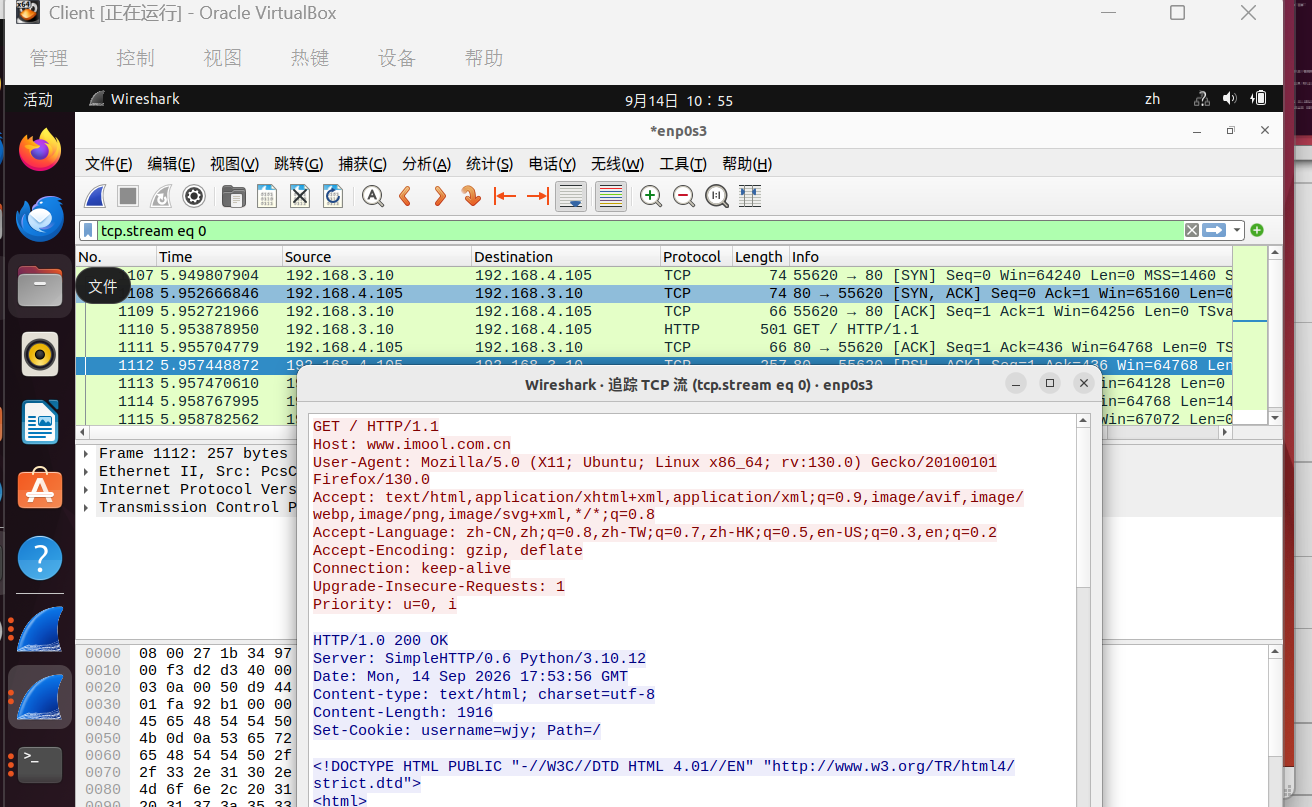
\includegraphics[width=0.8\textwidth]{figures/exp2_cookie.png}
    \caption{HTTP流量截图3}
    \label{fig:exp2_cookie}
\end{figure}

\subsection{特别关注的相关问题}
\subsubsection{域名解析过程涉及哪些IP包，请求和响应分别是什么}
虚拟机 Client （192.168.3.10） 向 DNS Server （192.168.2.53） 发送 DNS 查询请求，
请求解析 www.imool.com.cn；DNS Server 返回请求的响应，将该域名解析为 Web Server 地址 192.168.4.105

\subsubsection{ARP解析过程中，网关的MAC地址是什么}
根据 Wireshark 捕获到的 ARP Response（ARP 响应），默认网关 192.168.3.1 的 MAC 地址为：\\
08:00:27:1b:34:97

\subsubsection{Client 与 www.imool.com.cn 的连接建立和拆除过程}
TCP 连接建立采用三次握手：
192.168.3.10 → 192.168.4.105    [SYN]
192.168.4.105 → 192.168.3.10    [SYN, ACK]
192.168.3.10 → 192.168.4.105    [ACK]

TCP 连接拆除采用四次挥手为：
Client → Web Server       FIN, ACK
Web Server → Client       ACK
Web Server → Client       FIN, ACK
Client → Web Server       ACK

\subsubsection{使用 Wireshark 的协议流追踪功能提取 Cookie 信息}
在 Wireshark 中选择 HTTP 数据流并使用 TCP Stream（TCP 流）追踪功能，
可以观察到服务器返回的：
\begin{lstlisting}[language=bash,caption={cookie的显示}]
Set-Cookie: username=wjy; Path=/
\end{lstlisting}
其中 Cookie 名称为 username，值为 wjy，路径为 /。

\subsection{实验小结}
这一小节实验在实验一网络拓扑的基础上重新配置 DNS Server 和 Web Server，
并利用 OpenWRT 实现不同子网之间的路由通信。
通过 Wireshark 对访问 www.imool.com.cn 的全过程进行抓包，
观察了 DNS 域名解析、ARP 地址解析、TCP 三次握手和四次挥手以及 HTTP 请求和响应过程，
并通过 TCP 流追踪提取了 Cookie 信息。
通过本实验，我们对浏览器访问一个 Web 网站过程中各层协议之间的配合关系有了更加直观的认识。

% 实验三：使用 Scapy 构造 ICMP Echo Request
% 在此填写 Scapy 代码、报文字段、Victim 侧抓包结果和分析。
\section{实验三：使用 Scapy 构造 ICMP Echo Request}



\section{实验讨论}
% 在此填写实验讨论、问题分析和个人思考。

\section{参考资料}
% 直接引用请使用 \verb|\labquote[页码]{文献键}|；实际参考过的资料写入 references.bib。
\printbibliography[heading=none]

\section{附录：关键代码}
% 在此填写或使用 \lstinputlisting 引入完整、可运行、带注释的关键代码。

\end{document}
